
\chapter{Methodenentwicklung} % (fold)
\label{cha:methodenentwicklung}

Bild einer Biene in Abbildung \ref{fig:bee}.

\begin{figure}[h]
    \centering
    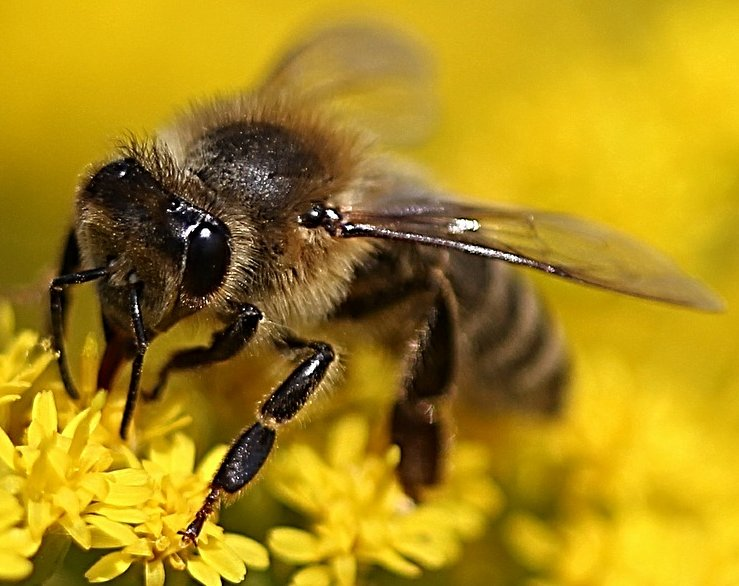
\includegraphics[width=\textwidth,keepaspectratio]{bee-593920_1920.jpg}
    \caption[Biene]{Apis Melferia - Frontalansicht einer Biene.}
    \label{fig:bee}
\end{figure}

Formeln im Text können mit Dollarzeichen dargestellt werden wie z. B. $x = 42$. Source code kann so wie in Listing \ref{lst:code} in Latex eingebaut werden, sollte jedoch nur wenige Zeilen haben.

\begin{lstlisting}[caption={Some example Code.}\label{lst:code},captionpos=b,language=Python] 
import numpy as np

def fun(x):
    return x + 1
\end{lstlisting}
